\section{Myplayer Class Reference}
\label{classMyplayer}\index{Myplayer@{Myplayer}}
{\tt \#include $<$Myplayer.h$>$}

Inheritance diagram for Myplayer:\begin{figure}[H]
\begin{center}
\leavevmode
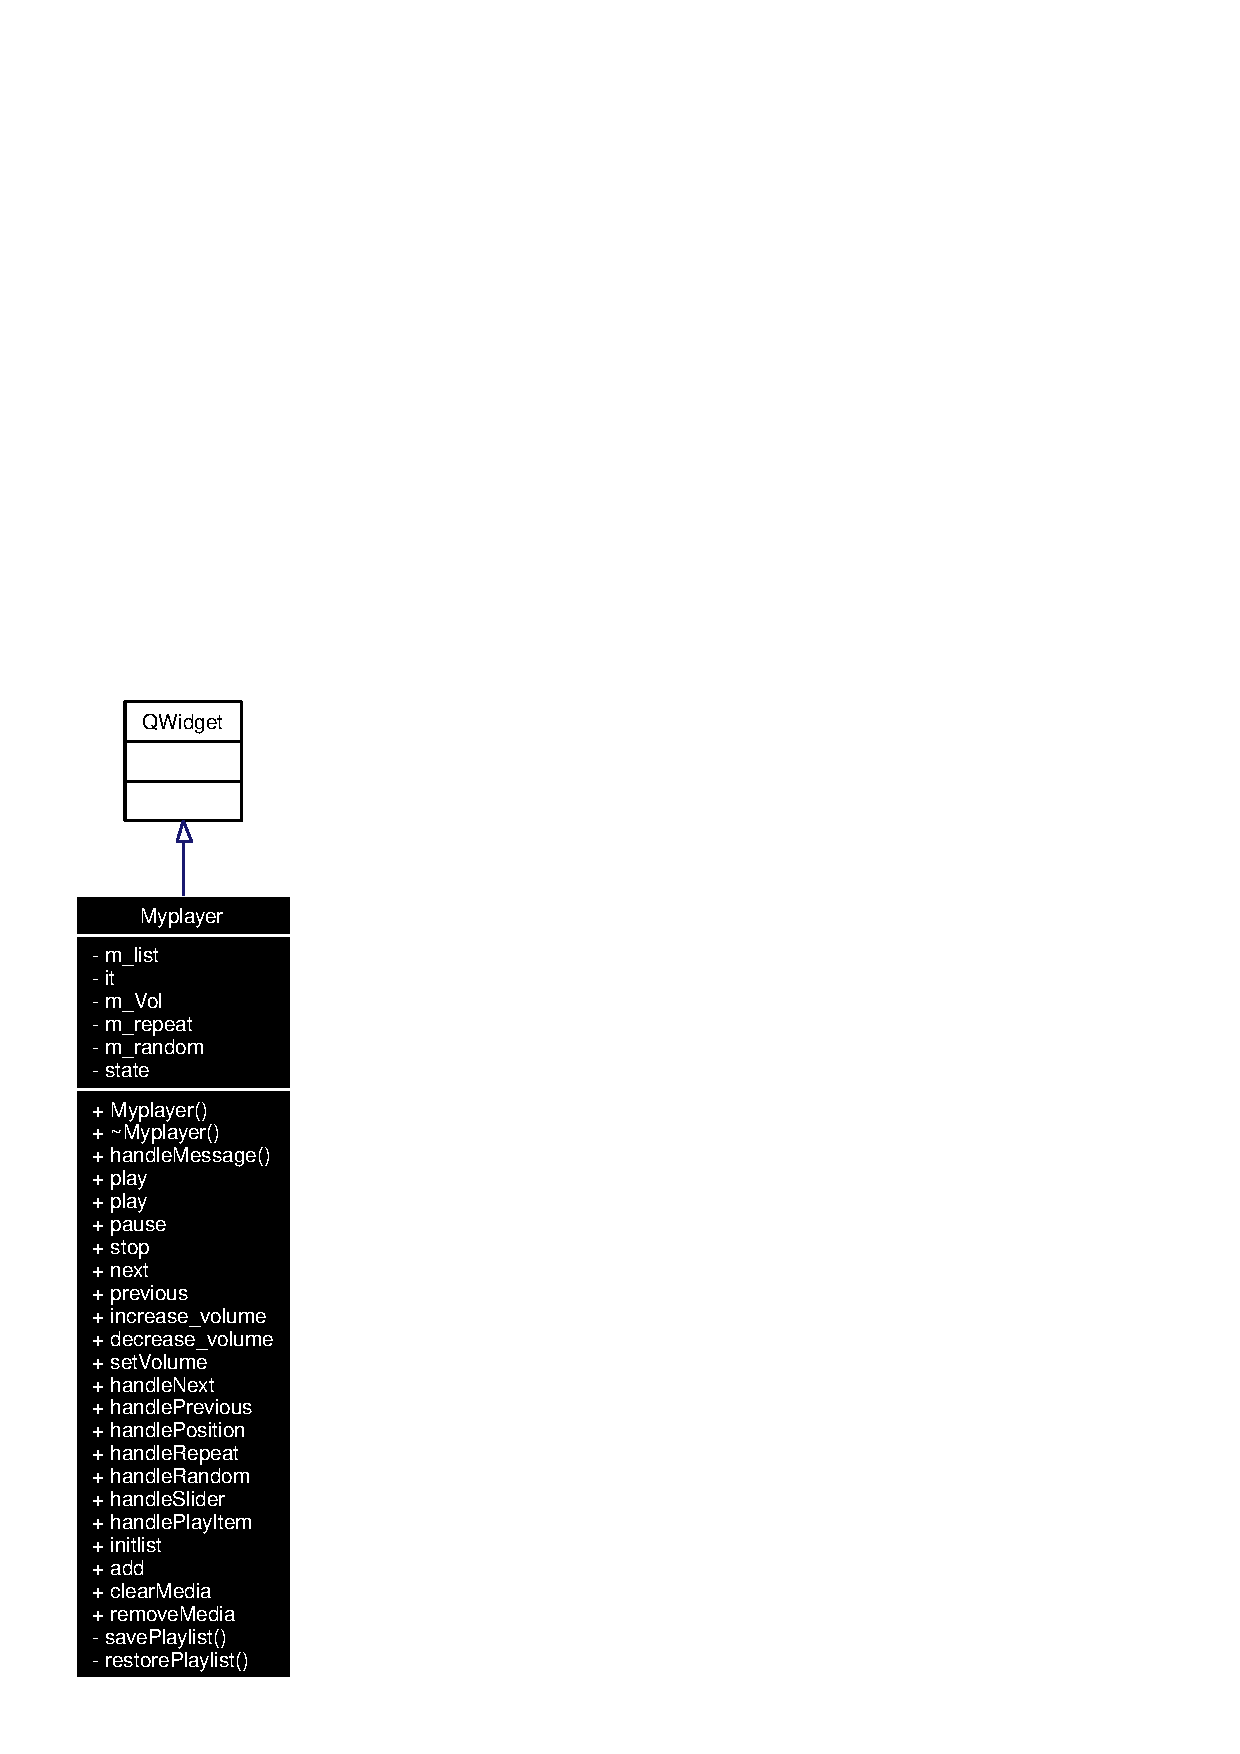
\includegraphics[width=70pt]{classMyplayer__inherit__graph}
\end{center}
\end{figure}
Collaboration diagram for Myplayer:\begin{figure}[H]
\begin{center}
\leavevmode
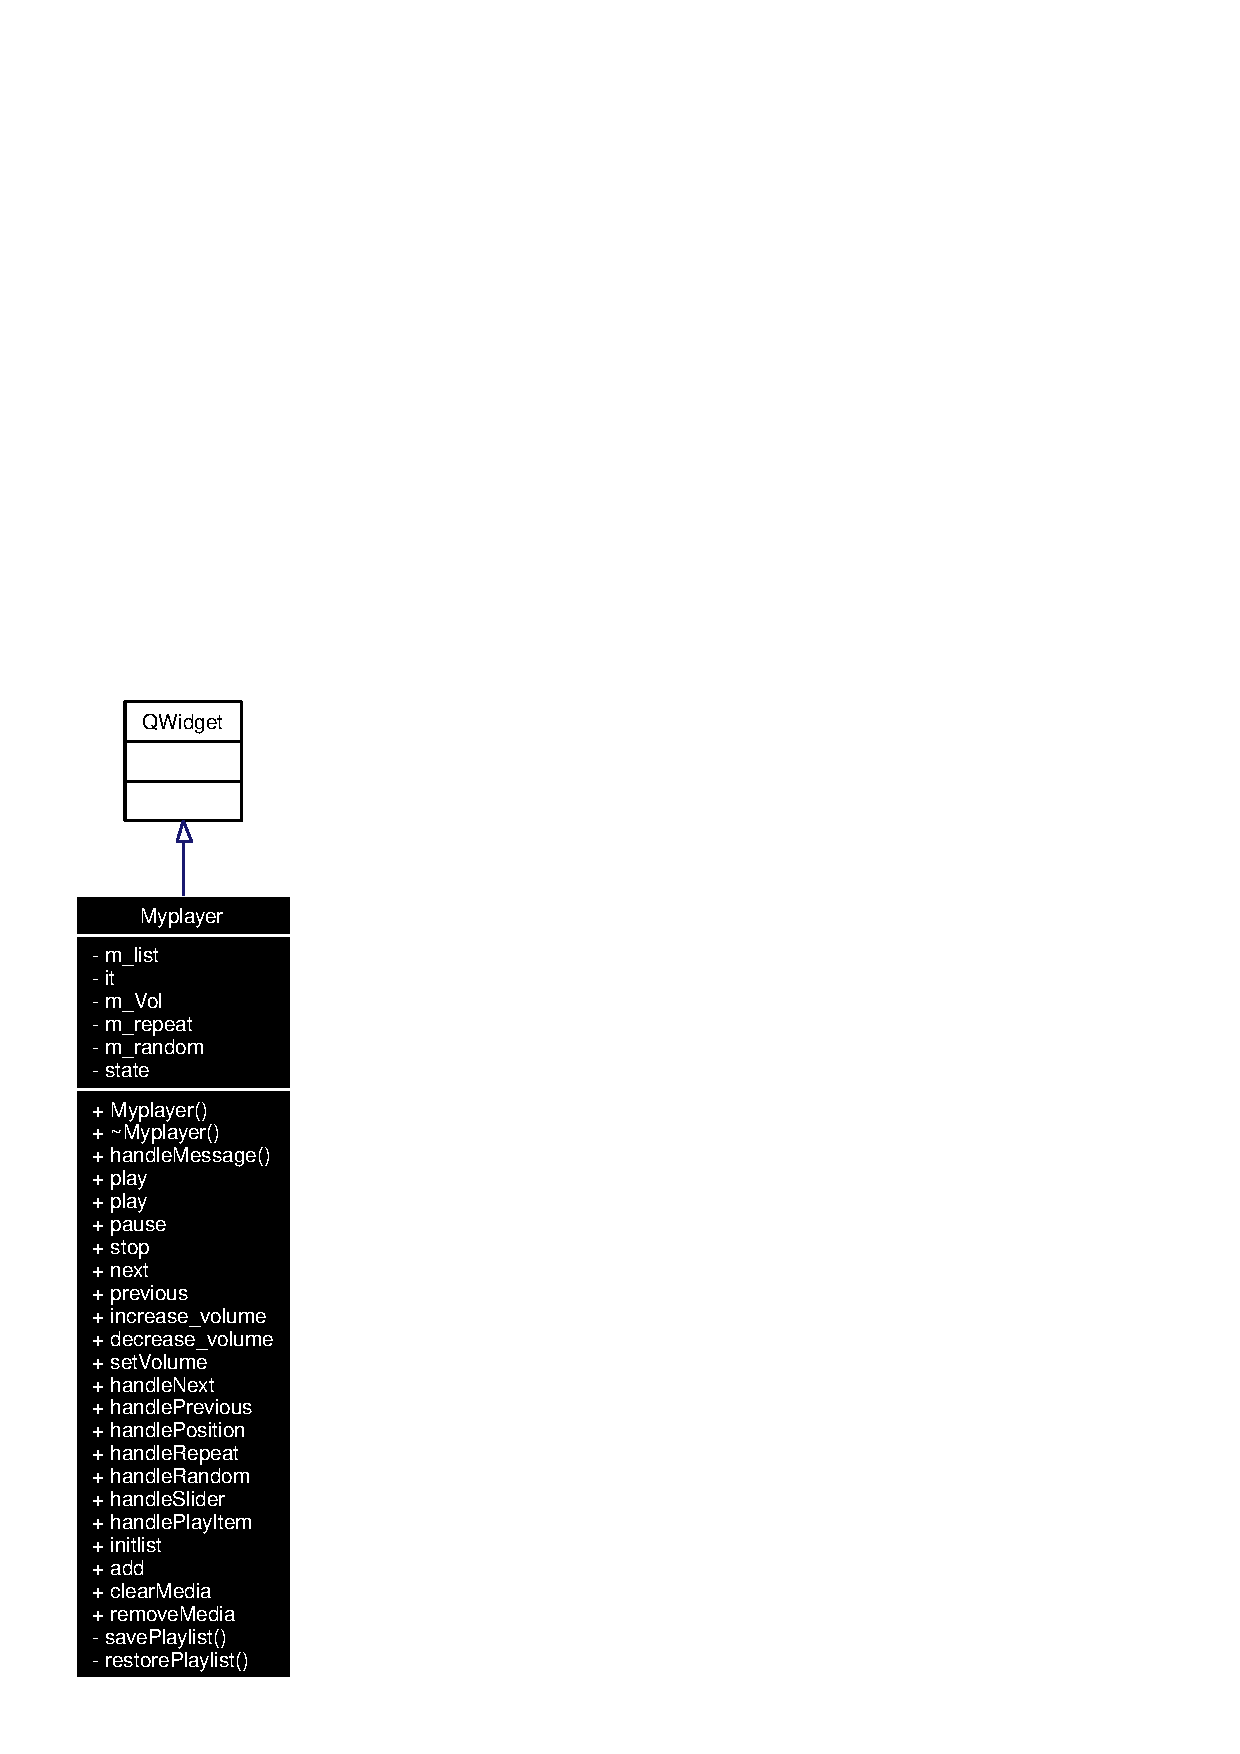
\includegraphics[width=70pt]{classMyplayer__coll__graph}
\end{center}
\end{figure}
\subsection*{Public Slots}
\begin{CompactItemize}
\item 
void {\bf play} ()
\item 
void {\bf play} (QString File\-Name)
\item 
void {\bf pause} ()
\item 
void {\bf stop} ()
\item 
void {\bf next} ()
\item 
void {\bf previous} ()
\item 
void {\bf increase\_\-volume} ()
\item 
void {\bf decrease\_\-volume} ()
\item 
void {\bf set\-Volume} (int)
\item 
void {\bf handle\-Next} ()
\item 
void {\bf handle\-Previous} ()
\item 
void {\bf handle\-Position} (int)
\item 
void {\bf handle\-Repeat} (bool)
\item 
void {\bf handle\-Random} (bool)
\item 
void {\bf handle\-Slider} (int)
\item 
void {\bf handle\-Play\-Item} (KURL \&)
\item 
void {\bf initlist} (KURL::List \&)
\item 
void {\bf add} (KURL::List \&)
\item 
void {\bf clear\-Media} ()
\item 
void {\bf remove\-Media} (KURL::List \&)
\end{CompactItemize}
\subsection*{Signals}
\begin{CompactItemize}
\item 
void {\bf track\-Message} (int, int, QString, QString, QString)
\item 
void {\bf volume\-Message} (int)
\item 
void {\bf position\-Message} (int)
\end{CompactItemize}
\subsection*{Public Member Functions}
\begin{CompactItemize}
\item 
{\bf Myplayer} ()
\item 
{\bf $\sim$Myplayer} ()
\item 
void {\bf handle\-Message} (const {\bf Meta\-Bundle} \&)
\end{CompactItemize}
\subsection*{Private Types}
\begin{CompactItemize}
\item 
enum {\bf PLAYSTATE} \{ {\bf Idle}, 
{\bf Pause}, 
{\bf Go}
 \}
\end{CompactItemize}
\subsection*{Private Member Functions}
\begin{CompactItemize}
\item 
void {\bf save\-Playlist} ()
\item 
void {\bf restore\-Playlist} ()
\end{CompactItemize}
\subsection*{Private Attributes}
\begin{CompactItemize}
\item 
KURL::List {\bf m\_\-list}
\item 
KURL::List::Iterator {\bf it}
\item 
int {\bf m\_\-Vol}
\item 
bool {\bf m\_\-repeat}
\item 
bool {\bf m\_\-random}
\item 
{\bf PLAYSTATE} {\bf state}
\end{CompactItemize}


\subsection{Member Enumeration Documentation}
\index{Myplayer@{Myplayer}!PLAYSTATE@{PLAYSTATE}}
\index{PLAYSTATE@{PLAYSTATE}!Myplayer@{Myplayer}}
\subsubsection{\setlength{\rightskip}{0pt plus 5cm}enum {\bf Myplayer::PLAYSTATE}\hspace{0.3cm}{\tt  [private]}}\label{classMyplayer_Myplayery3}


\begin{Desc}
\item[Enumeration values: ]\par
\begin{description}
\index{Idle@{Idle}!Myplayer@{Myplayer}}\index{Myplayer@{Myplayer}!Idle@{Idle}}\item[{\em 
Idle\label{classMyplayer_Myplayery3Myplayery0}
}]\index{Pause@{Pause}!Myplayer@{Myplayer}}\index{Myplayer@{Myplayer}!Pause@{Pause}}\item[{\em 
Pause\label{classMyplayer_Myplayery3Myplayery1}
}]\index{Go@{Go}!Myplayer@{Myplayer}}\index{Myplayer@{Myplayer}!Go@{Go}}\item[{\em 
Go\label{classMyplayer_Myplayery3Myplayery2}
}]\end{description}
\end{Desc}



Definition at line 30 of file Myplayer.h.



\footnotesize\begin{verbatim}31 {
32  Idle,Pause,Go
33 };
\end{verbatim}\normalsize 


\subsection{Constructor \& Destructor Documentation}
\index{Myplayer@{Myplayer}!Myplayer@{Myplayer}}
\index{Myplayer@{Myplayer}!Myplayer@{Myplayer}}
\subsubsection{\setlength{\rightskip}{0pt plus 5cm}Myplayer::Myplayer ()}\label{classMyplayer_Myplayera0}




Definition at line 31 of file Myplayer.cpp.

References handle\-Next(), handle\-Position(), handle\-Previous(), Engine\-Base::init(), Engine\-Base::init\-Mixer(), Engine\-Controller::instance(), m\_\-list, m\_\-random, m\_\-repeat, m\_\-Vol, Engine\-Base::set\-Default\-Sound\-Device(), Engine\-Controller::set\-Engine(), Engine\-Base::set\-Restore\-Effects(), Engine\-Base::set\-Sound\-Device(), Engine\-Base::set\-Sound\-Output(), Engine\-Base::set\-Volume(), and Engine\-Base::set\-Xfade\-Length().



\footnotesize\begin{verbatim}32 {
33      bool restartArts = false;
34      m_repeat = true;
35      m_random = false;
36      EngineBase* const engine = new ArtsEngine();
37      engine->init( restartArts, 9, true );//AmarokConfig::rememberEffects() );
38      engine->initMixer( false );//AmarokConfig::hardwareMixer() ); try to check the hardware mixer and use it 
39      engine->setVolume( 50 );
40      m_Vol = 50;
41      EngineController::setEngine( engine );
42      engine->setSoundOutput( "Alsa" );
43      engine->setSoundDevice( AmarokConfig::soundDevice() );
44      engine->setDefaultSoundDevice( !AmarokConfig::customSoundDevice() );
45      engine->setRestoreEffects( AmarokConfig::rememberEffects() );
46          //TODO deprecate/improve
47      engine->setXfadeLength( 2200 );
48      EngineController* const ec = EngineController::instance();
49      connect( ec, SIGNAL( orderNext() ), SLOT( handleNext() ) );
50      connect( ec, SIGNAL( orderPrevious() ), SLOT( handlePrevious() ) );      
51      connect(ec, SIGNAL(TrackPosition(int)), SLOT(handlePosition(int)) );
52      it = m_list.begin();
53 }
\end{verbatim}\normalsize 


Here is the call graph for this function:\begin{figure}[H]
\begin{center}
\leavevmode
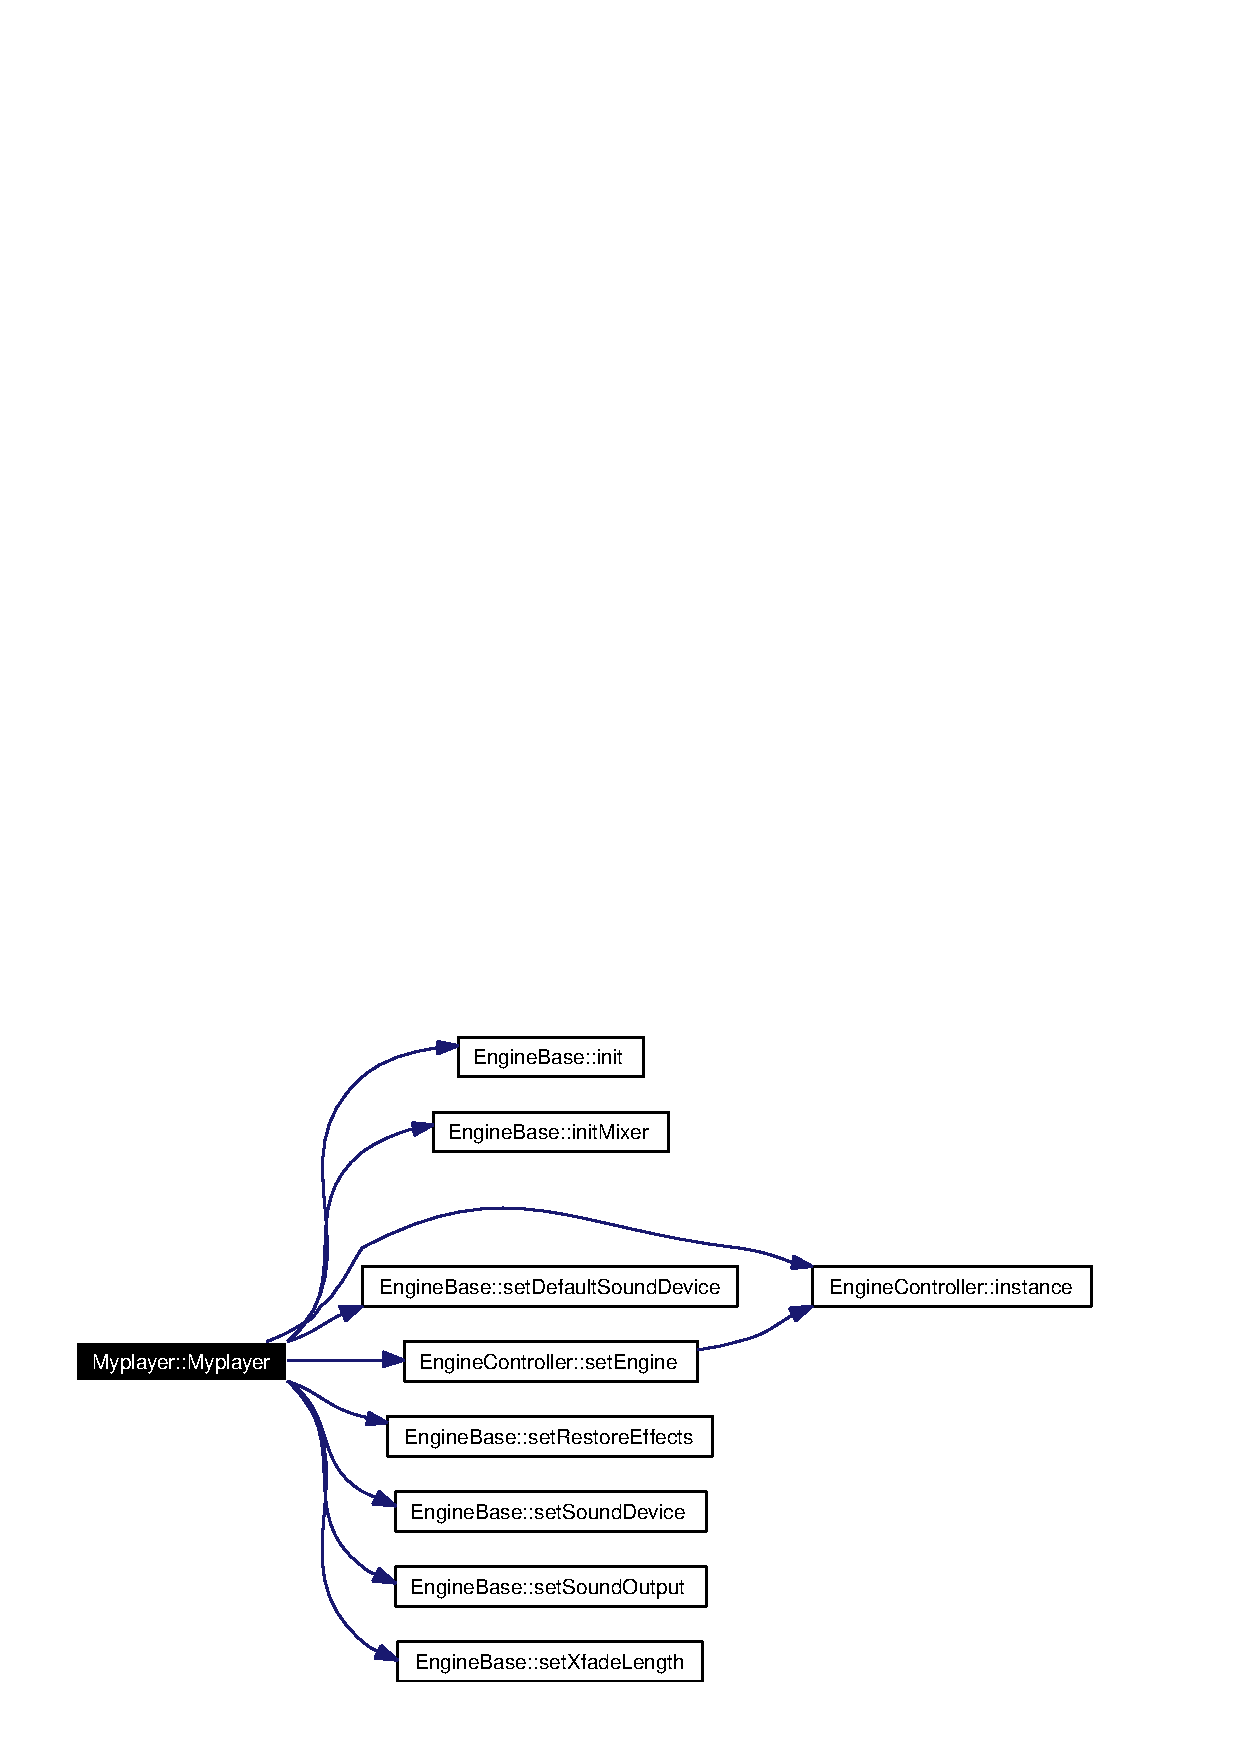
\includegraphics[width=262pt]{classMyplayer_Myplayera0_cgraph}
\end{center}
\end{figure}
\index{Myplayer@{Myplayer}!~Myplayer@{$\sim$Myplayer}}
\index{~Myplayer@{$\sim$Myplayer}!Myplayer@{Myplayer}}
\subsubsection{\setlength{\rightskip}{0pt plus 5cm}Myplayer::$\sim${\bf Myplayer} ()}\label{classMyplayer_Myplayera1}




Definition at line 55 of file Myplayer.cpp.



\footnotesize\begin{verbatim}56 {
57    kdDebug() << k_funcinfo << endl;
58 }
\end{verbatim}\normalsize 


\subsection{Member Function Documentation}
\index{Myplayer@{Myplayer}!add@{add}}
\index{add@{add}!Myplayer@{Myplayer}}
\subsubsection{\setlength{\rightskip}{0pt plus 5cm}void Myplayer::add (KURL::List \&)\hspace{0.3cm}{\tt  [slot]}}\label{classMyplayer_Myplayeri17}




Definition at line 267 of file Myplayer.cpp.

References m\_\-list.

Referenced by Sub\-Bar\-Player::insert\-Media().



\footnotesize\begin{verbatim}268 {     
269      if(!m_list.isEmpty())//Not Empty
270      {
271         kdDebug() << "PlayList is not empty !!" << endl;
272         KURL::List add_list = list;
273         for( KURL::List::ConstIterator add_it = add_list.begin();add_it != add_list.end();add_it++)
274         {
275               m_list.append( (*add_it).url() );
276         }       
277      }
278      else
279      {
280         m_list = list;
281         it = m_list.begin();
282         kdDebug() << "[Myplayer::add]: " << (*it).url() << endl;
283      }
284 }
\end{verbatim}\normalsize 
\index{Myplayer@{Myplayer}!clearMedia@{clearMedia}}
\index{clearMedia@{clearMedia}!Myplayer@{Myplayer}}
\subsubsection{\setlength{\rightskip}{0pt plus 5cm}void Myplayer::clear\-Media ()\hspace{0.3cm}{\tt  [slot]}}\label{classMyplayer_Myplayeri18}




Definition at line 286 of file Myplayer.cpp.

References m\_\-list.



\footnotesize\begin{verbatim}287 {    
288     if(m_list.isEmpty())kdDebug() << "[Myplayer::clearMedia]: it's empty"<< endl;
289     else{
290        m_list.clear();     
291        kdDebug() << "[Myplayer::clearMedia]: it's clear " << endl;      
292     }
293 }
\end{verbatim}\normalsize 
\index{Myplayer@{Myplayer}!decrease_volume@{decrease\_\-volume}}
\index{decrease_volume@{decrease\_\-volume}!Myplayer@{Myplayer}}
\subsubsection{\setlength{\rightskip}{0pt plus 5cm}void Myplayer::decrease\_\-volume ()\hspace{0.3cm}{\tt  [slot]}}\label{classMyplayer_Myplayeri7}




Definition at line 118 of file Myplayer.cpp.

References m\_\-Vol, and set\-Volume().



\footnotesize\begin{verbatim}119 {
120      setVolume(m_Vol-5);
121      kdDebug() << "[Myplayer]decrease_Vol --: " << endl;
122 }
\end{verbatim}\normalsize 
\index{Myplayer@{Myplayer}!handleMessage@{handleMessage}}
\index{handleMessage@{handleMessage}!Myplayer@{Myplayer}}
\subsubsection{\setlength{\rightskip}{0pt plus 5cm}void Myplayer::handle\-Message (const {\bf Meta\-Bundle} \&)}\label{classMyplayer_Myplayera2}




Definition at line 326 of file Myplayer.cpp.

References Meta\-Bundle::album(), Meta\-Bundle::artist(), Meta\-Bundle::bitrate(), Meta\-Bundle::length(), Meta\-Bundle::title(), and track\-Message().

Referenced by handle\-Next(), handle\-Previous(), and play().



\footnotesize\begin{verbatim}327 {
328     int m_length = bundle.length();
329     int m_bitrate = bundle.bitrate();
330     QString m_title = bundle.title();
331     QString m_artist = bundle.artist();
332     QString m_album = bundle.album();
333 
334     emit trackMessage(m_length,m_bitrate,m_title,m_artist,m_album);
335 }
\end{verbatim}\normalsize 


Here is the call graph for this function:\begin{figure}[H]
\begin{center}
\leavevmode
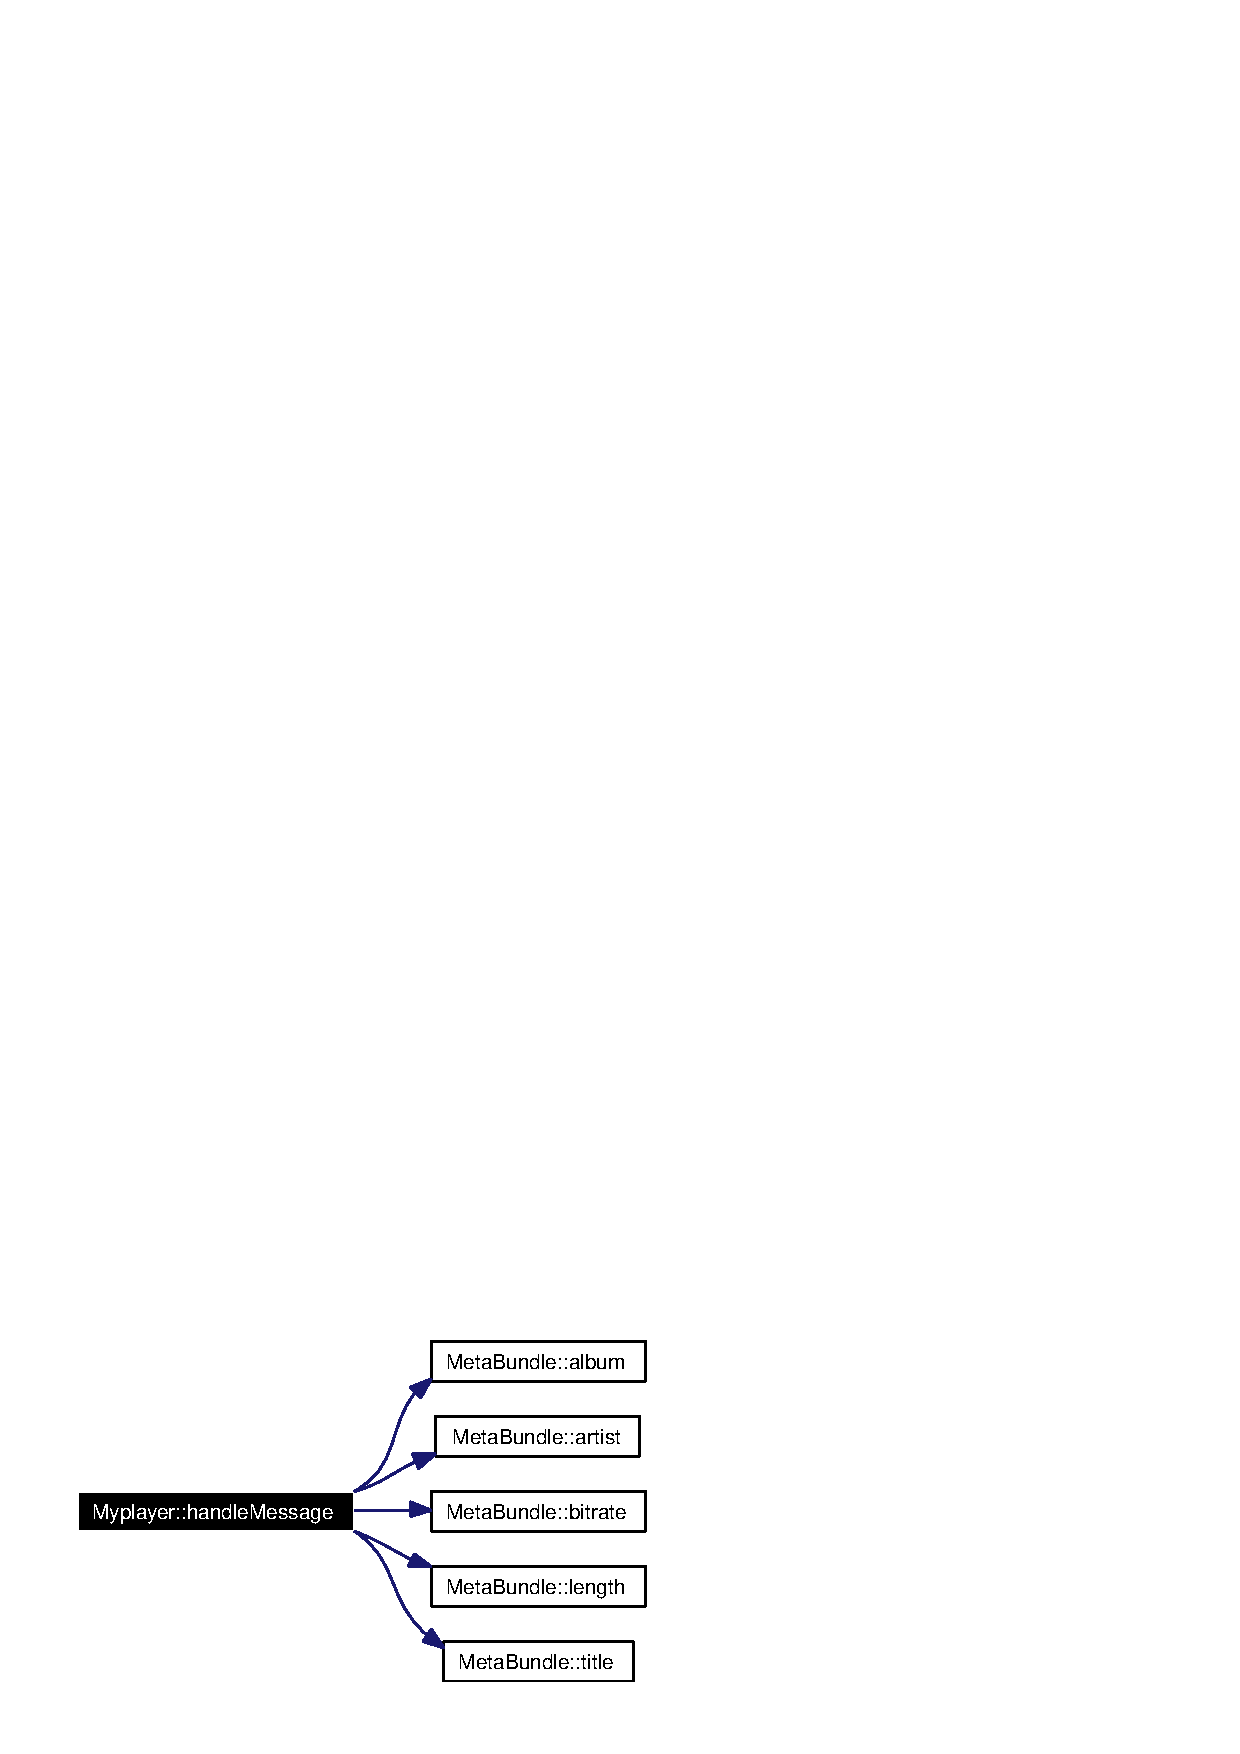
\includegraphics[width=155pt]{classMyplayer_Myplayera2_cgraph}
\end{center}
\end{figure}
\index{Myplayer@{Myplayer}!handleNext@{handleNext}}
\index{handleNext@{handleNext}!Myplayer@{Myplayer}}
\subsubsection{\setlength{\rightskip}{0pt plus 5cm}void Myplayer::handle\-Next ()\hspace{0.3cm}{\tt  [slot]}}\label{classMyplayer_Myplayeri9}




Definition at line 160 of file Myplayer.cpp.

References handle\-Message(), Engine\-Controller::instance(), m\_\-list, m\_\-random, m\_\-repeat, Engine\-Controller::play(), and Engine\-Controller::stop().

Referenced by Myplayer().



\footnotesize\begin{verbatim}161 {
162      kdDebug() << "[engine] hanleNext: " << endl;
163      if(m_random)
164      {
165       qWarning("Myplayer::random play item");
166        it = m_list.begin();
167        int randomNum = KApplication::random() % m_list.count();
168        for(int i = 0;it != m_list.end(); it++)
169        {
170          if(i == randomNum)break;
171          else i++;
172        }
173      }
174      else ++it;
175    
176      if(it != m_list.end())
177      {
178           EngineController::instance()->stop();
179           //kdDebug() << "[engine] play: " << (*it).url();
180           MetaBundle bundle( (*it).url() );  
181           EngineController::instance()->play(true,bundle);     
182           handleMessage(bundle);
183      }
184      else
185      {
186         
187         if(m_repeat)
188         {
189            it = m_list.begin();
190            qWarning("Myplayer::repeat play item");
191            MetaBundle bundle( (*it).url());
192            EngineController::instance()->play(true,bundle);
193            handleMessage(bundle);
194         }
195         
196         else 
197         {      
198              //  qWarning("=======================");
199              //  EngineController::instance()->stop();  
200            
201         }
202      }
203 }
\end{verbatim}\normalsize 
\index{Myplayer@{Myplayer}!handlePlayItem@{handlePlayItem}}
\index{handlePlayItem@{handlePlayItem}!Myplayer@{Myplayer}}
\subsubsection{\setlength{\rightskip}{0pt plus 5cm}void Myplayer::handle\-Play\-Item (KURL \&)\hspace{0.3cm}{\tt  [slot]}}\label{classMyplayer_Myplayeri15}




Definition at line 253 of file Myplayer.cpp.

References m\_\-list, and play().



\footnotesize\begin{verbatim}254 {
255      KURL::List::Iterator check_it = m_list.find(url);      
256      if(check_it != m_list.end())
257        {
258           it = check_it;
259           play();
260           kdDebug() << "Find Item "<< endl;
261        }
262      else kdDebug() << "NO this item!! " << endl;
263 }
\end{verbatim}\normalsize 
\index{Myplayer@{Myplayer}!handlePosition@{handlePosition}}
\index{handlePosition@{handlePosition}!Myplayer@{Myplayer}}
\subsubsection{\setlength{\rightskip}{0pt plus 5cm}void Myplayer::handle\-Position (int)\hspace{0.3cm}{\tt  [slot]}}\label{classMyplayer_Myplayeri11}




Definition at line 238 of file Myplayer.cpp.

References position\-Message().

Referenced by Myplayer(), and stop().



\footnotesize\begin{verbatim}239 {    
240      emit positionMessage(position);     
241 }
\end{verbatim}\normalsize 
\index{Myplayer@{Myplayer}!handlePrevious@{handlePrevious}}
\index{handlePrevious@{handlePrevious}!Myplayer@{Myplayer}}
\subsubsection{\setlength{\rightskip}{0pt plus 5cm}void Myplayer::handle\-Previous ()\hspace{0.3cm}{\tt  [slot]}}\label{classMyplayer_Myplayeri10}




Definition at line 205 of file Myplayer.cpp.

References handle\-Message(), Engine\-Controller::instance(), m\_\-list, and Engine\-Controller::play().

Referenced by Myplayer().



\footnotesize\begin{verbatim}206 {
207 //     EngineBase *engine = EngineController::engine();
208      kdDebug() << "[engine] hanlePrevious: " << endl;
209      if(it != m_list.begin())
210      {
211         --it;
212         MetaBundle bundle( (*it).url() );  
213 //      if(engine->state() == EngineBase::Playing)
214           EngineController::instance()->play(true,bundle); 
215         handleMessage(bundle);    
216      }
217      else
218      {
219         it = m_list.end();
220         --it;
221         MetaBundle bundle( (*it).url());
222 //      if(engine->state() == EngineBase::Playing)
223           EngineController::instance()->play(true,bundle);
224         handleMessage(bundle);
225      }
226 }
\end{verbatim}\normalsize 
\index{Myplayer@{Myplayer}!handleRandom@{handleRandom}}
\index{handleRandom@{handleRandom}!Myplayer@{Myplayer}}
\subsubsection{\setlength{\rightskip}{0pt plus 5cm}void Myplayer::handle\-Random (bool)\hspace{0.3cm}{\tt  [slot]}}\label{classMyplayer_Myplayeri13}




Definition at line 233 of file Myplayer.cpp.

References m\_\-random.



\footnotesize\begin{verbatim}234 {
235      m_random = random;
236 }
\end{verbatim}\normalsize 
\index{Myplayer@{Myplayer}!handleRepeat@{handleRepeat}}
\index{handleRepeat@{handleRepeat}!Myplayer@{Myplayer}}
\subsubsection{\setlength{\rightskip}{0pt plus 5cm}void Myplayer::handle\-Repeat (bool)\hspace{0.3cm}{\tt  [slot]}}\label{classMyplayer_Myplayeri12}




Definition at line 228 of file Myplayer.cpp.

References m\_\-repeat.

Referenced by Sub\-Bar\-Player::init\-Media(), and Sub\-Bar\-Player::insert\-Media().



\footnotesize\begin{verbatim}229 {
230      m_repeat = repeat;      
231 }
\end{verbatim}\normalsize 
\index{Myplayer@{Myplayer}!handleSlider@{handleSlider}}
\index{handleSlider@{handleSlider}!Myplayer@{Myplayer}}
\subsubsection{\setlength{\rightskip}{0pt plus 5cm}void Myplayer::handle\-Slider (int)\hspace{0.3cm}{\tt  [slot]}}\label{classMyplayer_Myplayeri14}




Definition at line 243 of file Myplayer.cpp.

References Engine\-Controller::engine(), and Engine\-Base::seek().

Referenced by Sub\-Bar\-Player::handle\-Next\-Released(), Sub\-Bar\-Player::handle\-Previous\-Released(), and Sub\-Bar\-Player::handle\-Slider\-Released().



\footnotesize\begin{verbatim}244 {
245      kdDebug() << "[Myplayer]sliderValue: "<< sliderValue << endl;
246      EngineBase *engine = EngineController::engine();
247      //if ( engine->state() == EngineBase::Playing )
248     // {
249         engine->seek( sliderValue*1000 );
250 //     }
251 }
\end{verbatim}\normalsize 
\index{Myplayer@{Myplayer}!increase_volume@{increase\_\-volume}}
\index{increase_volume@{increase\_\-volume}!Myplayer@{Myplayer}}
\subsubsection{\setlength{\rightskip}{0pt plus 5cm}void Myplayer::increase\_\-volume ()\hspace{0.3cm}{\tt  [slot]}}\label{classMyplayer_Myplayeri6}




Definition at line 112 of file Myplayer.cpp.

References m\_\-Vol, and set\-Volume().



\footnotesize\begin{verbatim}113 {
114      setVolume(m_Vol+5);        
115      kdDebug() << "[Myplayer]increase_Vol ++: " << endl;
116 }
\end{verbatim}\normalsize 
\index{Myplayer@{Myplayer}!initlist@{initlist}}
\index{initlist@{initlist}!Myplayer@{Myplayer}}
\subsubsection{\setlength{\rightskip}{0pt plus 5cm}void Myplayer::initlist (KURL::List \&)\hspace{0.3cm}{\tt  [slot]}}\label{classMyplayer_Myplayeri16}




Definition at line 364 of file Myplayer.cpp.

References m\_\-list.

Referenced by Sub\-Bar\-Player::init\-Media().



\footnotesize\begin{verbatim}365 {
366   m_list=list;
367   it = m_list.begin();
368   kdDebug() << "[Myplayer::add]: " << (*it).url() << endl;
369 }
\end{verbatim}\normalsize 
\index{Myplayer@{Myplayer}!next@{next}}
\index{next@{next}!Myplayer@{Myplayer}}
\subsubsection{\setlength{\rightskip}{0pt plus 5cm}void Myplayer::next ()\hspace{0.3cm}{\tt  [slot]}}\label{classMyplayer_Myplayeri4}




Definition at line 134 of file Myplayer.cpp.

References Engine\-Controller::instance(), m\_\-list, Engine\-Controller::next(), and Engine\-Controller::stop().



\footnotesize\begin{verbatim}135 {
136      if(!m_list.isEmpty())//DAVID Check list empty
137      {
138        EngineController::instance()->next();
139        kdDebug() << "[engine] Next: " << endl;
140      }
141      else 
142      {
143      
144        EngineController::instance()->stop();
145      }
146 }
\end{verbatim}\normalsize 
\index{Myplayer@{Myplayer}!pause@{pause}}
\index{pause@{pause}!Myplayer@{Myplayer}}
\subsubsection{\setlength{\rightskip}{0pt plus 5cm}void Myplayer::pause ()\hspace{0.3cm}{\tt  [slot]}}\label{classMyplayer_Myplayeri2}




Definition at line 106 of file Myplayer.cpp.

References Engine\-Controller::instance(), and Engine\-Controller::pause().



\footnotesize\begin{verbatim}107 {
108      EngineController::instance()->pause();
109      kdDebug() << "[engine] Pause: " << endl;
110 }
\end{verbatim}\normalsize 
\index{Myplayer@{Myplayer}!play@{play}}
\index{play@{play}!Myplayer@{Myplayer}}
\subsubsection{\setlength{\rightskip}{0pt plus 5cm}void Myplayer::play (QString {\em File\-Name})\hspace{0.3cm}{\tt  [slot]}}\label{classMyplayer_Myplayeri1}




Definition at line 76 of file Myplayer.cpp.

References handle\-Message(), Engine\-Controller::instance(), m\_\-list, and Engine\-Controller::play().



\footnotesize\begin{verbatim}77 {
78    bool find=false;
79    //DAVID Find file with filename
80    for( KURL::List::ConstIterator find_it = m_list.begin();find_it != m_list.end();find_it++)
81    {
82       if((*find_it).fileName()==filename)
83       {
84         //DAVID Find it
85         find=true;
86         it=m_list.find(*find_it);
87       }
88    }
89    if(find)
90    {
91        MetaBundle bundle( (*it).url() );        
92        EngineController::instance()->play(true,bundle); 
93        handleMessage(bundle);
94        kdDebug() << "[engine] play: " << endl;            
95    }
96    else qWarning("File Not Find!!");//this situation should not be happend
97 
98 }
\end{verbatim}\normalsize 
\index{Myplayer@{Myplayer}!play@{play}}
\index{play@{play}!Myplayer@{Myplayer}}
\subsubsection{\setlength{\rightskip}{0pt plus 5cm}void Myplayer::play ()\hspace{0.3cm}{\tt  [slot]}}\label{classMyplayer_Myplayeri0}




Definition at line 61 of file Myplayer.cpp.

References handle\-Message(), Engine\-Controller::instance(), m\_\-list, Engine\-Controller::play(), and Engine\-Controller::stop().

Referenced by handle\-Play\-Item().



\footnotesize\begin{verbatim}62 {          
63      if(!m_list.isEmpty())
64      {
65        MetaBundle bundle( (*it).url() );        
66        EngineController::instance()->play(bundle); 
67        handleMessage(bundle);
68        kdDebug() << "[engine] play: " << endl;            
69      }
70      else
71      {
72         EngineController::instance()->stop();
73         kdDebug() << "[engine] Stop: " << endl;            
74      }
75 }
\end{verbatim}\normalsize 
\index{Myplayer@{Myplayer}!positionMessage@{positionMessage}}
\index{positionMessage@{positionMessage}!Myplayer@{Myplayer}}
\subsubsection{\setlength{\rightskip}{0pt plus 5cm}void Myplayer::position\-Message (int)\hspace{0.3cm}{\tt  [signal]}}\label{classMyplayer_Myplayerl2}




Definition at line 195 of file Myplayer.moc.

Referenced by handle\-Position().



\footnotesize\begin{verbatim}196 {
197     activate_signal( staticMetaObject()->signalOffset() + 2, t0 );
198 }
\end{verbatim}\normalsize 
\index{Myplayer@{Myplayer}!previous@{previous}}
\index{previous@{previous}!Myplayer@{Myplayer}}
\subsubsection{\setlength{\rightskip}{0pt plus 5cm}void Myplayer::previous ()\hspace{0.3cm}{\tt  [slot]}}\label{classMyplayer_Myplayeri5}




Definition at line 148 of file Myplayer.cpp.

References Engine\-Controller::instance(), m\_\-list, Engine\-Controller::previous(), and Engine\-Controller::stop().



\footnotesize\begin{verbatim}149 {
150      if(!m_list.isEmpty())
151      {
152        EngineController::instance()->previous();
153        kdDebug() << "[engine] Previous: "<< endl;
154      }
155      else EngineController::instance()->stop();
156      
157 }
\end{verbatim}\normalsize 
\index{Myplayer@{Myplayer}!removeMedia@{removeMedia}}
\index{removeMedia@{removeMedia}!Myplayer@{Myplayer}}
\subsubsection{\setlength{\rightskip}{0pt plus 5cm}void Myplayer::remove\-Media (KURL::List \&)\hspace{0.3cm}{\tt  [slot]}}\label{classMyplayer_Myplayeri19}




Definition at line 295 of file Myplayer.cpp.

References m\_\-list.

Referenced by Sub\-Bar\-Player::remove\-Media().



\footnotesize\begin{verbatim}296 {       
297     KURL::List::ConstIterator check_it;
298         
299     if(m_list.isEmpty())kdDebug() << "[Myplayer::removeMedia]: it's empty"<< endl;
300     else{
301                 for( KURL::List::ConstIterator remove_it = remove_list.begin();remove_it != remove_list.end();remove_it++)
302                 {
303                         check_it = m_list.find((*remove_it).url());      
304                         if(check_it != m_list.end())
305                         {
306                                 m_list.remove((*check_it).url());
307                                 kdDebug() << "Remove Item "<< endl;
308                         }
309                         else kdDebug() << "NO this item!! " << endl;
310                 }
311         
312                 for( KURL::List::ConstIterator refresh_it = m_list.begin();refresh_it != m_list.end();refresh_it++)  
313                 {
314                         if((*refresh_it).isEmpty())
315                         {
316                                 for(check_it = refresh_it; check_it != m_list.end();)
317                                 (*check_it).url() = (*(check_it++)).url();                  
318                         }         
319                 }
320                 it = m_list.begin();   
321     } 
322 }
\end{verbatim}\normalsize 
\index{Myplayer@{Myplayer}!restorePlaylist@{restorePlaylist}}
\index{restorePlaylist@{restorePlaylist}!Myplayer@{Myplayer}}
\subsubsection{\setlength{\rightskip}{0pt plus 5cm}void Myplayer::restore\-Playlist ()\hspace{0.3cm}{\tt  [private]}}\label{classMyplayer_Myplayerd1}




Definition at line 351 of file Myplayer.cpp.

References m\_\-list.



\footnotesize\begin{verbatim}352 {
353     QFile file( "file.txt" );
354     if ( file.open( IO_ReadOnly ) ) {
355         QTextStream stream( &file );            
356         while ( !stream.atEnd() ) {
357              KURL url(stream.readLine()); // line of text excluding '\n'         
358              m_list << url;
359         }
360         kdDebug() << "Load Playlist "<< endl;
361         file.close();
362     }
363 }
\end{verbatim}\normalsize 
\index{Myplayer@{Myplayer}!savePlaylist@{savePlaylist}}
\index{savePlaylist@{savePlaylist}!Myplayer@{Myplayer}}
\subsubsection{\setlength{\rightskip}{0pt plus 5cm}void Myplayer::save\-Playlist ()\hspace{0.3cm}{\tt  [private]}}\label{classMyplayer_Myplayerd0}




Definition at line 339 of file Myplayer.cpp.

References m\_\-list.



\footnotesize\begin{verbatim}340 {
341     QFile file( "file.txt" );
342     if ( file.open( IO_WriteOnly ) ) {
343         QTextStream stream( &file );
344           for(KURL::List::Iterator save_it = m_list.begin(); save_it != m_list.end(); ++save_it)
345             stream << (*save_it).url() << "\n";
346         file.close();
347 kdDebug() << "save file finished!!"<< endl;     
348     }    
349 }
\end{verbatim}\normalsize 
\index{Myplayer@{Myplayer}!setVolume@{setVolume}}
\index{setVolume@{setVolume}!Myplayer@{Myplayer}}
\subsubsection{\setlength{\rightskip}{0pt plus 5cm}void Myplayer::set\-Volume (int)\hspace{0.3cm}{\tt  [slot]}}\label{classMyplayer_Myplayeri8}




Definition at line 124 of file Myplayer.cpp.

References Engine\-Controller::instance(), m\_\-Vol, Engine\-Controller::set\-Volume(), and volume\-Message().

Referenced by decrease\_\-volume(), and increase\_\-volume().



\footnotesize\begin{verbatim}125 {
126      if( percent < 0 ) m_Vol = 0;
127      else if( percent > 100) m_Vol = 100;
128      else m_Vol = percent;
129      EngineController::instance()->setVolume(m_Vol);
130      emit volumeMessage(m_Vol);
131      kdDebug() << "[Myplayer]setVolume: " << m_Vol << endl;
132 }
\end{verbatim}\normalsize 
\index{Myplayer@{Myplayer}!stop@{stop}}
\index{stop@{stop}!Myplayer@{Myplayer}}
\subsubsection{\setlength{\rightskip}{0pt plus 5cm}void Myplayer::stop ()\hspace{0.3cm}{\tt  [slot]}}\label{classMyplayer_Myplayeri3}




Definition at line 99 of file Myplayer.cpp.

References handle\-Position(), Engine\-Controller::instance(), and Engine\-Controller::stop().



\footnotesize\begin{verbatim}100 {     
101      EngineController::instance()->stop();
102      handlePosition(0);
103      kdDebug() << "[engine] Stop: " << endl;
104 }
\end{verbatim}\normalsize 
\index{Myplayer@{Myplayer}!trackMessage@{trackMessage}}
\index{trackMessage@{trackMessage}!Myplayer@{Myplayer}}
\subsubsection{\setlength{\rightskip}{0pt plus 5cm}void Myplayer::track\-Message (int, int, QString, QString, QString)\hspace{0.3cm}{\tt  [signal]}}\label{classMyplayer_Myplayerl0}




Definition at line 172 of file Myplayer.moc.

Referenced by handle\-Message().



\footnotesize\begin{verbatim}173 {
174     if ( signalsBlocked() )
175         return;
176     QConnectionList *clist = receivers( staticMetaObject()->signalOffset() + 0 );
177     if ( !clist )
178         return;
179     QUObject o[6];
180     static_QUType_int.set(o+1,t0);
181     static_QUType_int.set(o+2,t1);
182     static_QUType_QString.set(o+3,t2);
183     static_QUType_QString.set(o+4,t3);
184     static_QUType_QString.set(o+5,t4);
185     activate_signal( clist, o );
186 }
\end{verbatim}\normalsize 
\index{Myplayer@{Myplayer}!volumeMessage@{volumeMessage}}
\index{volumeMessage@{volumeMessage}!Myplayer@{Myplayer}}
\subsubsection{\setlength{\rightskip}{0pt plus 5cm}void Myplayer::volume\-Message (int)\hspace{0.3cm}{\tt  [signal]}}\label{classMyplayer_Myplayerl1}




Definition at line 189 of file Myplayer.moc.

Referenced by set\-Volume().



\footnotesize\begin{verbatim}190 {
191     activate_signal( staticMetaObject()->signalOffset() + 1, t0 );
192 }
\end{verbatim}\normalsize 


\subsection{Member Data Documentation}
\index{Myplayer@{Myplayer}!it@{it}}
\index{it@{it}!Myplayer@{Myplayer}}
\subsubsection{\setlength{\rightskip}{0pt plus 5cm}KURL::List::Iterator {\bf Myplayer::it}\hspace{0.3cm}{\tt  [private]}}\label{classMyplayer_Myplayerr1}




Definition at line 74 of file Myplayer.h.\index{Myplayer@{Myplayer}!m_list@{m\_\-list}}
\index{m_list@{m\_\-list}!Myplayer@{Myplayer}}
\subsubsection{\setlength{\rightskip}{0pt plus 5cm}KURL::List {\bf Myplayer::m\_\-list}\hspace{0.3cm}{\tt  [private]}}\label{classMyplayer_Myplayerr0}




Definition at line 73 of file Myplayer.h.

Referenced by add(), clear\-Media(), handle\-Next(), handle\-Play\-Item(), handle\-Previous(), initlist(), Myplayer(), next(), play(), previous(), remove\-Media(), restore\-Playlist(), and save\-Playlist().\index{Myplayer@{Myplayer}!m_random@{m\_\-random}}
\index{m_random@{m\_\-random}!Myplayer@{Myplayer}}
\subsubsection{\setlength{\rightskip}{0pt plus 5cm}bool {\bf Myplayer::m\_\-random}\hspace{0.3cm}{\tt  [private]}}\label{classMyplayer_Myplayerr4}




Definition at line 77 of file Myplayer.h.

Referenced by handle\-Next(), handle\-Random(), and Myplayer().\index{Myplayer@{Myplayer}!m_repeat@{m\_\-repeat}}
\index{m_repeat@{m\_\-repeat}!Myplayer@{Myplayer}}
\subsubsection{\setlength{\rightskip}{0pt plus 5cm}bool {\bf Myplayer::m\_\-repeat}\hspace{0.3cm}{\tt  [private]}}\label{classMyplayer_Myplayerr3}




Definition at line 76 of file Myplayer.h.

Referenced by handle\-Next(), handle\-Repeat(), and Myplayer().\index{Myplayer@{Myplayer}!m_Vol@{m\_\-Vol}}
\index{m_Vol@{m\_\-Vol}!Myplayer@{Myplayer}}
\subsubsection{\setlength{\rightskip}{0pt plus 5cm}int {\bf Myplayer::m\_\-Vol}\hspace{0.3cm}{\tt  [private]}}\label{classMyplayer_Myplayerr2}




Definition at line 75 of file Myplayer.h.

Referenced by decrease\_\-volume(), increase\_\-volume(), Myplayer(), and set\-Volume().\index{Myplayer@{Myplayer}!state@{state}}
\index{state@{state}!Myplayer@{Myplayer}}
\subsubsection{\setlength{\rightskip}{0pt plus 5cm}{\bf PLAYSTATE} {\bf Myplayer::state}\hspace{0.3cm}{\tt  [private]}}\label{classMyplayer_Myplayerr5}




Definition at line 78 of file Myplayer.h.

The documentation for this class was generated from the following files:\begin{CompactItemize}
\item 
{\bf Myplayer.h}\item 
{\bf Myplayer.moc}\item 
{\bf Myplayer.cpp}\end{CompactItemize}
